% ============================================================================
%  biosim-lab — "Nasıl çalışıyor", uzman olmayanlar için.
%  Derleme:  xelatex main-tr.tex  (içindekiler için iki kez)
%  Lisans: MIT, kodun geri kalanıyla aynı.
%  İngilizce sürüm: main.tex
% ============================================================================
\documentclass[11pt,a4paper]{article}

\usepackage{fontspec}
\setmainfont{STIX Two Text}
\setsansfont{Helvetica Neue}[Scale=MatchLowercase]
\setmonofont{Menlo}[Scale=0.86]
\usepackage{unicode-math}
\setmathfont{STIX Two Math}

\usepackage{polyglossia}
\setmainlanguage{turkish}
\setotherlanguage{english}

\usepackage[margin=2.4cm,top=2.2cm,bottom=2.4cm]{geometry}
\usepackage{amsmath}
\usepackage{graphicx}
\usepackage{booktabs}
\usepackage{array}
\usepackage{xcolor}
\usepackage{tcolorbox}
\usepackage{tikz}
\usepackage{pgfplots}
\usepackage{siunitx}
\usepackage{enumitem}
\usepackage{microtype}
\usepackage{caption}
\usepackage[hidelinks,bookmarksnumbered]{hyperref}
\usepackage{fancyhdr}

\pgfplotsset{compat=1.18}
\usetikzlibrary{arrows.meta,positioning,decorations.pathmorphing,decorations.markings,
                patterns,calc,shapes.geometric,fit,backgrounds}
\tcbuselibrary{skins,breakable}

\definecolor{blue1}{HTML}{2A78D6}
\definecolor{orange1}{HTML}{EB6834}
\definecolor{aqua1}{HTML}{1BAF7A}
\definecolor{red1}{HTML}{E34948}
\definecolor{ink}{HTML}{0B0B0B}
\definecolor{muted}{HTML}{52514E}
\definecolor{rule1}{HTML}{E6E5E1}
\definecolor{surface}{HTML}{FCFCFB}

\captionsetup{font=small,labelfont={bf,color=muted},textfont={color=muted}}
\setlist{itemsep=2pt,topsep=4pt,parsep=0pt}
\sisetup{per-mode=symbol,detect-all}

\pagestyle{fancy}\fancyhf{}
\renewcommand{\headrulewidth}{0.4pt}
\fancyhead[L]{\footnotesize\sffamily\color{muted}biosim-lab — nasıl çalışıyor}
\fancyhead[R]{\footnotesize\sffamily\color{muted}\thepage}

% --- kutular ----------------------------------------------------------------
\newtcolorbox{plain}[1][]{
  enhanced, breakable, colback=blue1!5, colframe=blue1!55, boxrule=0.6pt,
  arc=2pt, left=8pt, right=8pt, top=6pt, bottom=6pt,
  fonttitle=\sffamily\bfseries\small, coltitle=blue1!75!black,
  title={Düz anlatımla}, #1}

\newtcolorbox{analogy}[1][]{
  enhanced, breakable, colback=aqua1!6, colframe=aqua1!55, boxrule=0.6pt,
  arc=2pt, left=8pt, right=8pt, top=6pt, bottom=6pt,
  fonttitle=\sffamily\bfseries\small, coltitle=aqua1!55!black,
  title={Kafanızda tutacağınız resim}, #1}

\newtcolorbox{warnbox}[1][]{
  enhanced, breakable, colback=orange1!6, colframe=orange1!60, boxrule=0.6pt,
  arc=2pt, left=8pt, right=8pt, top=6pt, bottom=6pt,
  fonttitle=\sffamily\bfseries\small, coltitle=orange1!60!black,
  title={Bunun geçerli olmadığı yer}, #1}

\newtcolorbox{keybox}[1][]{
  enhanced, breakable, colback=surface, colframe=ink, boxrule=1pt,
  arc=2pt, left=8pt, right=8pt, top=7pt, bottom=7pt,
  fonttitle=\sffamily\bfseries\small, coltitle=ink,
  title={Asıl önemli olan denklem}, #1}

\newcommand{\sym}[2]{\textcolor{ink}{$#1$} & #2 \\}
\newcommand{\dims}[1]{\textcolor{muted}{\footnotesize [#1]}}

\title{\vspace{-1.2cm}\sffamily\bfseries
  \texttt{biosim-lab} Gerçekte Nasıl Çalışıyor\\[4pt]
  \large\mdseries Biyolojisi, fiziği, matematiği ve kodu ---\\
  \large\mdseries bunların hiçbirini bilmeyenler için anlatıldı}
\author{\sffamily\normalsize \texttt{biosim-lab} kaynak koduna eşlik eden belge}
\date{\sffamily\small\today}

\begin{document}
\maketitle
\thispagestyle{empty}

\begin{center}
\begin{minipage}{0.86\textwidth}
\small\color{muted}
\textbf{Bu belge kimin için.} ``Kanser hücresi'', ``ses dalgası'' ve
``simülasyon'' sözcüklerini duymuş ve bu yazılımın ne yaptığını, neden birinin
ona güvenmesi gerektiğini dürüstçe ve sırayla öğrenmek isteyen biri için.
Fizik, biyoloji ve programlama bilgisi varsayılmıyor. Her denklemin önünde onun
ne anlama geldiğini söyleyen bir cümle, hemen altında da her simgeyi tanımlayan
bir çizelge var. Hiçbir yerde ``gösterilebilir ki'' denip geçilmiyor.

\medskip
\textbf{Bu belge ne değil.} Sonuçların özeti değil. Yaklaşık beşte biri modelin
\emph{yanlış yaptığı} şeylere ayrılmıştır, çünkü okuyucunun geri kalan dörtte
beşe güvenip güvenmeyeceğine karar verebilmesi için asıl gereken kısım odur.

\medskip
\textbf{İngilizce sürüm:} \texttt{biosim-lab-explained.pdf}
\end{minipage}
\end{center}

\vfill
\begin{center}
\small\color{muted}
Kaynak kod: \texttt{biosim\_lab/} \quad$\cdot$\quad MIT lisansı \quad$\cdot$\quad
Buradaki her fiziksel sabit ya bir DOI ya da açık bir ``varsayım'' etiketi taşır
\end{center}
\clearpage

\tableofcontents
\clearpage

% ============================================================================
\part*{I. Bölüm --- Sorun, ve bu bir biyoloji sorunu}
\addcontentsline{toc}{part}{I. Bölüm --- Sorun, ve bu bir biyoloji sorunu}
\section{Beş milyar hücre arasında bir hücre bulmak}

İlerlemiş katı tümörü olan bir insan, o tümörden kan dolaşımına hücre salar.
Bunlara \textbf{dolaşan tümör hücreleri} ya da kısaca CTC denir. Üç nedenden
önemlidirler: sayıları hastalığın gidişatını izler, tümörün \emph{bugün} hangi
mutasyonları taşıdığını görmek için dizilenebilirler (biyopsi gününde
taşıdıklarını değil), ve elde etmek için bir organa iğne sokmak yerine yalnızca
kan almak yeterlidir.

Zorluk aritmetiktir. Bir mililitre kanda kabaca şunlar bulunur:

\begin{center}
\small
\begin{tabular}{lrl}
\toprule
\textbf{Hücre} & \textbf{Mililitredeki sayı} & \textbf{Ne yapar} \\
\midrule
Alyuvarlar (eritrositler) & $5\,000\,000\,000$ & oksijen taşır \\
Trombositler             & $250\,000\,000$    & yaraları pıhtılaştırır \\
Akyuvarlar (lökositler)  & $7\,000\,000$      & bağışıklık sistemi \\
\textbf{Dolaşan tümör hücreleri} & \textbf{yaklaşık 1} & aradığınız şey \\
\bottomrule
\end{tabular}
\end{center}

\begin{plain}
Beş milyar hücre arasından belirli bir tanesini arıyorsunuz. Kan hücreleri kum
taneleri olsaydı, tek bir belirli taneyi bulmak için tenis kortu büyüklüğünde
bir sahili taramanız gerekirdi --- üstelik onu zedelemeden, çünkü sonrasında
üretip dizilemek istiyorsunuz.
\end{plain}

İki yaklaşım ailesi var.

\textbf{Kimyasal.} Manyetik boncukları, tümör hücrelerinde bulunup kan
hücrelerinde bulunmayan bir proteine yapışan antikorla kaplayın, karıştırın ve
boncukları mıknatısla çekin. Bu yöntem çalışır ve onaylı klinik testlerin
temelidir. Zayıflığı şudur: yalnızca sizin seçtiğiniz proteini taşıyan hücreleri
yakalar --- ve en tehlikeli tümör hücreleri, yani yolculuk edebilmek için kimlik
değiştirmiş olanlar, tam da o proteini kapatmış olanlardır.

\textbf{Fiziksel.} Kimyayı tümüyle bir kenara bırakın. Tümör hücreleri kan
hücrelerinden basitçe \emph{daha büyüktür}. Boyuta göre ayırın. Bir boyut
süzgecinden kaçmak için kapatılabilecek hiçbir şey yoktur.

Bu yazılım fiziksel bir ayırıcıyı simüle eder ve kullandığı fiziksel özellik
sestir.

\section{Bir fizikçi için hücre nedir}

Biyolojiyi bir an için soyun. Bu yazılımdaki denklemler açısından bir hücre
şudur:

\begin{center}
\small
\begin{tabular}{lp{10.2cm}}
\toprule
\textbf{Bir küre} & yarıçapı $r$, \SI{1}{\micro\meter} (bir trombosit) ile
\SI{10}{\micro\meter} (bir tümör hücresi) arasında. Bir insan saçı yaklaşık
\SI{70}{\micro\meter} kalınlığındadır. \\[3pt]
\textbf{Sudan biraz ağır} & yoğunluk $\rho_p$,
\SI{1050}{\kilogram\per\cubic\meter} ile
\SI{1100}{\kilogram\per\cubic\meter} arasında; su
\SI{997}{\kilogram\per\cubic\meter}. Yani \%5--10 daha ağır. \\[3pt]
\textbf{Sudan biraz daha zor sıkışır} & sıkıştırılabilirlik $\kappa_p$ yaklaşık
$3{,}7\times10^{-10}\,\si{\per\pascal}$; su
$4{,}48\times10^{-10}\,\si{\per\pascal}$. Yani yaklaşık \%20 daha sert. \\
\bottomrule
\end{tabular}
\end{center}

Fiziksel tanımın tamamı bu. Üç sayı: ne kadar büyük, ne kadar ağır, ne kadar
sert. Bu simülasyonun akustikle yaptığı her şey bu üçünden ve başka hiçbir
şeyden çıkar.

\begin{warnbox}
Gerçek bir hücre türdeş jelden yapılmış bir küre değildir. Bir zarı, geri
kalanından daha yoğun bir çekirdeği ve ittiğinizde değişen bir biçimi vardır.
Onu türdeş bir küre saymak akustik soru için iyi, başka sorular için kötü
çalışan bir yaklaşıklıktır. Bunun bedeli \S\ref{sec:limits}'te sıralanmıştır.
\end{warnbox}

\subsection*{Varsayılan simülasyondaki hücreler}

\begin{center}
\small
\begin{tabular}{llrrrl}
\toprule
\textbf{Anahtar} & \textbf{Hücre} & $r$ \dims{\si{\micro\meter}} &
$\rho_p$ \dims{\si{\kilogram\per\cubic\meter}} &
$\kappa_p$ \dims{$10^{-10}\,\si{\per\pascal}$} & \textbf{Rolü} \\
\midrule
\texttt{mcf7} & MCF-7 meme kanseri & 9,00 & 1068 & 3,72 & hedef \\
\texttt{rbc}  & alyuvar            & 2,78 & 1099 & 3,41 & arka plan \\
\texttt{wbc}  & akyuvar            & 4,25 & 1070 & 3,99 & arka plan \\
\texttt{platelet} & trombosit      & 1,19 & 1058 & 3,13 & arka plan \\
\midrule
\multicolumn{2}{l}{\emph{karşılaştırma için su}} & --- & 997 & 4,48 & \\
\bottomrule
\end{tabular}
\end{center}

MCF-7, 1970'te bir hastadan alınıp o günden beri laboratuvarlarda üretilen bir
meme kanseri hücre hattıdır. Burada kullanılmasının nedeni, akustik ayrım
makalelerinin kullandığı hat olması ve dolayısıyla ölçülmüş özelliklerinin
literatürde bulunmasıdır.

\begin{plain}
Sayıların ne kadar benzer olduğuna dikkat edin. Bir tümör hücresiyle bir alyuvar
yoğunlukta \%3, sertlikte \%9 farklıdır. Farklar bunlardan ibaret olsaydı hiçbir
ayırıcı çalışmazdı. Bizi kurtaran ilk sütundur: tümör hücresi \textbf{3,2 kat
daha geniştir} --- ve göreceğimiz gibi, genişlik üçüncü kuvvete yükseltilen
özelliktir.
\end{plain}

\subsection*{Hücrelerin hepsi aynı boyda değildir}

Gerçek popülasyonların bir dağılımı vardır. ``\SI{9}{\micro\meter}'lik'' bir
tümör hücresi demek, \SI{9}{\micro\meter} çevresinde bir dağılım demektir.
Yazılım her simüle edilen hücrenin yarıçapını \textbf{log-normal} bir dağılımdan
çeker --- hücre boyu histogramları için standart görgül biçim, ve negatif
yarıçap üretemeyen bir dağılım.

\begin{equation}
r \sim \operatorname{LogNormal}(\mu,\sigma), \qquad
\sigma^2=\ln\!\left(1+\mathrm{CV}^2\right), \qquad
\mu=\ln \bar r-\tfrac{1}{2}\sigma^2 .
\end{equation}

\begin{center}\small
\begin{tabular}{ll}
\sym{\bar r}{istediğiniz ortalama yarıçap, örneğin \SI{9}{\micro\meter}}
\sym{\mathrm{CV}}{yayılım, ortalamanın kesri olarak: 0,12 demek $\pm\%12$ demek}
\sym{\mu,\sigma}{log-normal formülünün gerçekte istediği parametreler; yukarıdaki
iki satır bildiğinizi istediğine çevirir}
\end{tabular}
\end{center}

Bu göründüğünden önemlidir. Ayırma kuvveti $r^3$ ile ölçeklendiğinden,
ortalamadan \%12 küçük bir hücre ortalama kuvvetin $0{,}88^3 = \%68$'ini
hisseder. Hücre boyutundaki yayılım, bir ayırıcının hiçbir zaman \%100 saf
olmamasının başlıca nedenidir.

% ============================================================================
\clearpage
\part*{II. Bölüm --- Hile, ve bu bir fizik}
\addcontentsline{toc}{part}{II. Bölüm --- Hile, ve bu bir fizik}

\section{Ses sıkıştırmaktır}

Ses, suyun içinden geçen bir madde değildir. Suyun içinden geçen bir sıkışma ve
gevşeme örüntüsüdür. Sıvının herhangi bir noktasında basınç saniyede milyonlarca
kez biraz artar, biraz azalır, tekrar artar.

Onu üç sayı tanımlar:

\begin{center}\small
\begin{tabular}{ll}
\sym{f}{\textbf{frekans} --- saniyede kaç kez sıkışma yinelendiği. Bizimki
\SI{6,632}{\mega\hertz}: saniyede 6,6 milyon kez, insanın duyabildiği en tiz
sesin yaklaşık 300 katı.}
\sym{c}{\textbf{ses hızı} --- örüntünün ne kadar hızlı ilerlediği. Suda
\SI{1497}{\meter\per\second}, havadakinin dört katı.}
\sym{\lambda}{\textbf{dalga boyu} --- bir sıkışmayla bir sonraki arasındaki
uzaklık, $\lambda = c/f$.}
\end{tabular}
\end{center}

\begin{plain}
Frekans ne kadar \emph{hızlı} titreştiğidir. Dalga boyu titreşimlerin ne kadar
\emph{aralıklı} olduğudur. Ses hızı ikisini birbirine kilitler: birini seçtiniz
mi öbürü belli olur.
\end{plain}

\section{Duran dalgalar: hiçbir şeyin kımıldamadığı yer}

Bir kanalda dalga gönderin ve geri sekmesine izin verin. Giden ve dönen dalgalar
toplanır. Bazı yerlerde her zaman birbirlerini götürürler, bazı yerlerde her
zaman güçlendirirler. Örüntü ilerlemeyi bırakır ve yerinde nabız gibi atarak
durur. Buna \textbf{duran dalga} denir.

\begin{analogy}
Bir atlama ipinin bir ucunu siz, öbür ucunu bir arkadaşınız tutsun ve doğru
hızda sallayın. İp öyle bir biçime oturur ki bazı noktalar şiddetle inip
çıkarken bazı noktalar --- \emph{düğümler} --- hiç kımıldamaz. İp hiçbir yere
gitmiyor. Duruyor.

Kanaldaki ses de aynısını yapar, yalnız salınan şey yükseklik değil basınçtır.
Basıncın hiç değişmediği yerler (\textbf{basınç düğümleri}, sessiz yerler) ve en
sert salındığı yerler (\textbf{karın noktaları}, gürültülü yerler) vardır.
\end{analogy}

\begin{figure}[h]
\centering
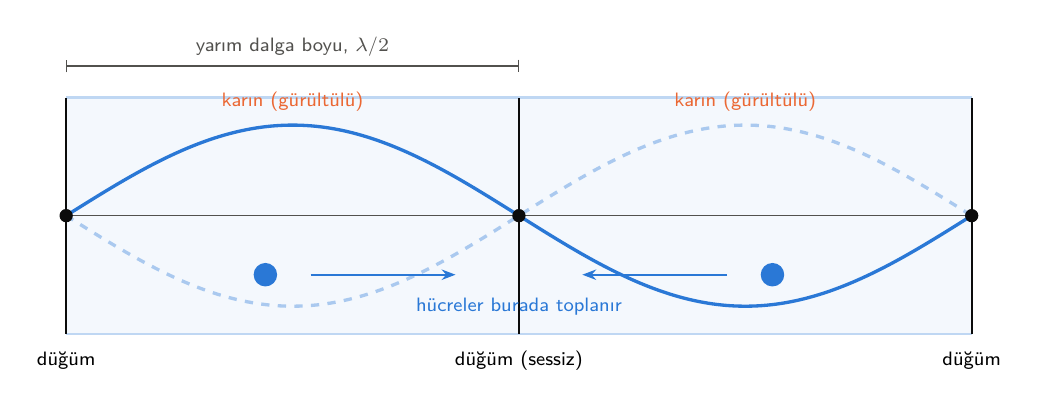
\begin{tikzpicture}[x=1.15cm,y=1cm]
  \fill[blue1!5] (0,-1.5) rectangle (10,1.5);
  \draw[blue1!30,thick] (0,-1.5) -- (10,-1.5);
  \draw[blue1!30,thick] (0,1.5) -- (10,1.5);
  \draw[blue1,very thick,domain=0:10,samples=200] plot (\x,{1.15*sin(deg(pi*\x/5))});
  \draw[blue1!40,very thick,dashed,domain=0:10,samples=200]
        plot (\x,{-1.15*sin(deg(pi*\x/5))});
  \draw[muted,thin] (0,0) -- (10,0);
  \foreach \x in {0,5,10}{
    \draw[ink,thick] (\x,-1.5) -- (\x,1.5);
    \node[circle,fill=ink,inner sep=1.7pt] at (\x,0) {};
  }
  \node[below,font=\scriptsize\sffamily] at (0,-1.6) {düğüm};
  \node[below,font=\scriptsize\sffamily] at (5,-1.6) {düğüm (sessiz)};
  \node[below,font=\scriptsize\sffamily] at (10,-1.6) {düğüm};
  \node[above,font=\scriptsize\sffamily,orange1] at (2.5,1.2) {karın (gürültülü)};
  \node[above,font=\scriptsize\sffamily,orange1] at (7.5,1.2) {karın (gürültülü)};
  \node[circle,fill=blue1,inner sep=3pt] (c1) at (2.2,-0.75) {};
  \node[circle,fill=blue1,inner sep=3pt] (c2) at (7.8,-0.75) {};
  \draw[-{Stealth[length=5pt]},blue1,thick] (2.7,-0.75) -- (4.3,-0.75);
  \draw[-{Stealth[length=5pt]},blue1,thick] (7.3,-0.75) -- (5.7,-0.75);
  \node[font=\scriptsize\sffamily,blue1] at (5,-1.15) {hücreler burada toplanır};
  \draw[|-|,muted] (0,1.9) -- (5,1.9)
      node[midway,above,font=\scriptsize\sffamily,color=muted]
      {yarım dalga boyu, $\lambda/2$};
\end{tikzpicture}
\caption{Kanal boyunca duran bir basınç dalgası. Düz ve kesikli eğriler basınç
salınımının iki uç noktasıdır. Düğümlerde basınç hiç değişmez; karın
noktalarında en sert salınır. Sudan daha yoğun ve daha sert olan hücreler ---
yani vücuttaki her hücre --- düğümlere doğru sürüklenir.}
\end{figure}

Komşu düğümler arasındaki aralık her zaman dalga boyunun \emph{yarısıdır}. Bu
tek olgu cihazı tasarlamamızı sağlar: dalga boyunu seçtiniz mi, hücrelerin
nerede toplanacağını seçmişsiniz demektir.

\section{Duran dalga neden bir şeyi iter}

İşte gerçekten şaşırtıcı olan kısım. Düğümdeki basınç hiç değişmez. Öyleyse
düğümün az ötesinde duran bir hücre neden herhangi bir itme hissetsin?

Yanıt şu: hücre sesi \emph{saçar}. Çevresindeki sudan daha yoğun ve daha
serttir, bu yüzden sıvıyla tam uyum içinde hareket etmez. Kendi küçük dalgasını
yeniden yayar ve o saçılan dalga özgün dalgayla girişir. Salınımın tam bir
çevrimi boyunca ortalama alındığında --- ki bu 150 nanosaniye sürer, dolayısıyla
hücrenin yaşadığı her şey için ``ortalama'' adil bir tanımdır --- girişim sıfıra
gitmez. Geriye küçük ve sürekli bir itme kalır.

\begin{analogy}
Kanalın üzerine serilmiş görünmez bir tepeler ve vadiler manzarası düşünün.
Üzerine konan bir hücre, tıpkı bir bilye gibi, yokuş aşağı yuvarlanır. Ses onu
sürüklemiyor; ses onu bir eğimin üzerine oturtmuş.

Bu manzaranın teknik adı, 1962'de hesaplayan Sovyet fizikçisinden geliyor:
\textbf{Gor'kov potansiyeli}. Vadilerin nerede olduğu --- sessiz düğümlerde mi,
gürültülü karınlarda mı --- hücreye bağlıdır.
\end{analogy}

Bu manzaranın herhangi bir noktadaki yüksekliği şudur:

\begin{equation}
U = V_c\left[\;\underbrace{\frac{f_1}{2}\,\kappa_f\,\langle p^2\rangle}_{\text{sıkışmadan}}
\;-\;\underbrace{\frac{3}{4}\,f_2\,\rho_f\,\langle v^2\rangle}_{\text{çalkalanmadan}}\;\right]
\label{eq:gorkov}
\end{equation}

\begin{center}\small
\begin{tabular}{ll}
\sym{U}{o noktadaki manzaranın yüksekliği \dims{joule}}
\sym{V_c}{hücrenin hacmi, $\tfrac{4}{3}\pi r^3$ \dims{\si{\cubic\meter}}}
\sym{\langle p^2\rangle}{orada basıncın ne kadar sert salındığı, çevrim ortalaması}
\sym{\langle v^2\rangle}{orada suyun ileri geri ne kadar sert çalkalandığı, ortalaması}
\sym{\rho_f,\kappa_f}{suyun yoğunluğu ve sıkıştırılabilirliği}
\sym{f_1,f_2}{hücrenin sudan ne kadar farklı olduğunu anlatan iki sayı --- sonraki bölüm}
\end{tabular}
\end{center}

Kuvvet ise yalnızca manzaranın ne kadar dik olduğudur:

\begin{equation}
\boxed{\;F = -\nabla U\;}
\end{equation}

$\nabla$ (``nabla'' ya da ``grad'') yalnızca \emph{eğim} demektir. Eksi işareti
yokuş aşağı demektir. Hepsi bu: manzarayı kurun, eğimini ölçün, kuvveti
buldunuz.

\begin{plain}
Ses alanı görünmez, engebeli bir yüzey yaratır. Hücreler onun üzerinde yokuş
aşağı yuvarlanır. Denklem~\eqref{eq:gorkov}'deki iki terim, hücrenin yerini
aldığı sudan farklı olmasının iki nedenidir: sıkıştırılmaya farklı direnir
(birinci terim) ve sarsılmaya farklı direnir (ikinci terim).
\end{plain}

\section{Kontrast faktörü: iki soru, tek sayı}

Hücrenin yalnızca iki soruyu yanıtlaması gerekir.

\begin{center}\small
\begin{tabular}{p{4.3cm}p{5.1cm}p{5.2cm}}
\toprule
\textbf{Soru} & \textbf{Sayısı} & \textbf{Tipik bir hücre için} \\
\midrule
Sudan daha mı zor sıkışıyorum? &
$f_1 = 1 - \dfrac{\kappa_p}{\kappa_f}$ (\emph{monopol} terimi) &
$f_1 = 1 - \frac{3{,}72}{4{,}48} = 0{,}169$, yani evet, biraz \\[10pt]
Sudan daha mı ağırım? &
$f_2 = \dfrac{2(\rho_p-\rho_f)}{2\rho_p+\rho_f}$ (\emph{dipol} terimi) &
$f_2 = \frac{2(1068-997)}{2136+997} = 0{,}045$, yani evet, azıcık \\
\bottomrule
\end{tabular}
\end{center}

İkisini tek bir \textbf{akustik kontrast faktöründe} birleştirin:

\begin{equation}
\Phi \;=\; f_1 + \tfrac{3}{2}f_2
\;=\; \frac{5\rho_p-2\rho_f}{2\rho_p+\rho_f}-\frac{\kappa_p}{\kappa_f}
\label{eq:phi}
\end{equation}

\begin{center}\small
\begin{tabular}{ll}
\sym{\Phi>0}{hücre sudan hem daha yoğun \emph{hem} daha serttir.
\textbf{Düğüme} gider. İnsan vücudundaki her hücre bunu yapar.}
\sym{\Phi<0}{hücre daha hafif ya da daha yumuşaktır. \textbf{Karın noktasına}
gider. Yağ damlacıkları ve gaz kabarcıkları bunu yapar.}
\sym{\Phi=0}{cisim akustik olarak sudan ayırt edilemez ve hiçbir şey olmaz.}
\end{tabular}
\end{center}

\begin{center}\small
\begin{tabular}{lrl}
\toprule
\textbf{Parçacık} & $\Phi$ & \textbf{Nereye gider} \\
\midrule
trombosit & $+0{,}360$ & düğüm \\
alyuvar & $+0{,}334$ & düğüm \\
MCF-7 tümör hücresi & $+0{,}237$ & düğüm \\
akyuvar & $+0{,}179$ & düğüm \\
yağ damlacığı & $-0{,}273$ & \textbf{karın} \\
\bottomrule
\end{tabular}
\end{center}

Yağ damlacığı çizelgede bilerek duruyor: sınama durumudur.
Denklem~\eqref{eq:phi}'in doğru yazılmış her uygulaması onun için \emph{eksi}
bir sayı döndürmek \emph{zorundadır} ve otomatik test paketi tam olarak bunu
denetler.

\begin{warnbox}
\textbf{Üç kat tuzağı.} Yayımlanmış literatürde $\Phi$'nin iki tanımı dolaşır ve
tam olarak üç kat farklıdırlar. Yukarıdaki klasik olanıdır. Bazı yazarlar
(en çok atıf alan modern ders yazısı dahil) $\Phi_{\text{alt}} = f_1/3 + f_2/2 =
\Phi/3$ kullanır ve bunu telafi eden bir çarpanı olan bir kuvvet formülüyle
birlikte verirler.

İkisini karıştırırsanız hesapladığınız her kuvvet 3 kat yanlış olur --- ve
inandırıcı görünür, çünkü büyüklük mertebesi hâlâ doğrudur. Yazılım ikisini de
farklı adlarla sunar ve test paketi oranlarını tam olarak 3'e sabitler.
\end{warnbox}

\section{Bütün cihazın üzerine kurulduğu tek denklem}

Bir boyutlu duran dalga için denklem~\eqref{eq:gorkov} üzerinde eğim hesabı
yapmak şunu verir:

\begin{keybox}
\begin{equation}
F_r(x) \;=\; -\,\frac{\pi\, p_0^{\,2}\, V_c\, \kappa_f}{2\lambda}\;\Phi\;
\sin\!\big(2k(x-x_{\text{düğüm}})\big)
\label{eq:force}
\end{equation}
\vspace{-4pt}
\begin{center}\small
\begin{tabular}{ll}
\sym{F_r}{hücreye yandan gelen itme \dims{newton}}
\sym{x}{hücrenin nerede olduğu, kanal boyunca ölçülür}
\sym{x_{\text{düğüm}}}{en yakın sessiz noktanın nerede olduğu}
\sym{p_0}{sesin ne kadar gürültülü olduğu (basınç genliği) \dims{pascal}}
\sym{V_c}{hücrenin hacmi $=\tfrac43\pi r^3$}
\sym{\kappa_f}{suyun ne kadar sıkışabildiği}
\sym{\lambda}{duran dalganın dalga boyu}
\sym{k}{$=2\pi/\lambda$; dalga boyunun fizikçilerin yeğlediği yazılışı}
\sym{\Phi}{denklem~\eqref{eq:phi}'deki kontrast faktörü}
\end{tabular}
\end{center}
\end{keybox}

Parça parça okuyun.

\begin{itemize}
\item \textbf{$\sin(2k(x-x_{\text{düğüm}}))$} --- yön. Tam düğümde ve tam karın
noktasında sıfırdır, bir yanda artı öbür yanda eksidir. Yani hücre her zaman
düğüme doğru itilir ve oraya vardığında kuvvet kapanır. Orada park eder.
\item \textbf{$p_0^2$} --- sesi iki kat yükseltin, itme dört katına çıkar. İki
katına değil. Sürüş voltajının bu kadar etkili bir düğme olmasının nedeni budur.
\item \textbf{$V_c \propto r^3$} --- \emph{cihazın tamamı budur} ve kendi
bölümünü hak eder.
\item \textbf{$\Phi$} --- hücrenin hangi yöne ve ne kadar güçlü tepki verdiği.
\item \textbf{$1/\lambda$} --- daha sık bir örüntü daha sert iter, çünkü manzara
daha dik eğimlere sahiptir.
\end{itemize}

\section{Boyut neden kazanır: $r^2$ yasası}
\label{sec:r2}

Hücre boşlukta değildir. Sudadır ve su direnir. Bu direnç \textbf{Stokes
sürüklenmesidir}:

\begin{equation}
F_d = 6\pi\mu r\,(u_f - u_p)
\label{eq:stokes}
\end{equation}

\begin{center}\small
\begin{tabular}{ll}
\sym{\mu}{sıvının ne kadar koyu olduğu (viskozite); su
\SI{0,89e-3}{\pascal\second}}
\sym{r}{hücrenin yarıçapı --- dikkat: hacim değil, \textbf{yarıçap}}
\sym{u_f-u_p}{hücrenin çevresindeki suya göre ne kadar hızlı gittiği}
\end{tabular}
\end{center}

Şimdi ikisini birleştirin. Hücre, itmeyle sürüklenme dengeleninceye kadar
hızlanır; bu neredeyse anında olur (bkz.\ \S\ref{sec:lowre}). Dengede:

\begin{equation}
\underbrace{\;\text{itme} \;\propto\; r^3\;}_{\text{denklem \eqref{eq:force}}}
\;=\;
\underbrace{\;\text{sürüklenme} \;\propto\; r \times \text{hız}\;}_{\text{denklem \eqref{eq:stokes}}}
\qquad\Longrightarrow\qquad
\boxed{\ \text{hız} \;\propto\; r^2\ }
\end{equation}

\begin{plain}
İtme hücrenin \emph{hacmiyle} büyür. Direnç yalnızca \emph{yarıçapıyla} büyür.
Hacim yarıçapı yener. Yarıçapı iki katına çıkarın, hücre dört kat hızlı hareket
etsin.
\end{plain}

\begin{analogy}
Bir bilyeyi ve bir gülleyi havuza bırakın. İkisi de yerçekimini bütün
hacimleriyle, suyun direncini yalnızca genişlikleri boyunca hisseder. Gülle
kazanır, hem de az farkla değil. Akustik ayırma tam olarak budur: yerçekimi
yerine ses, aşağı yerine yana.
\end{analogy}

Gerçek sayıları koyun. Bir MCF-7 tümör hücresini bir alyuvarla karşılaştırırsak:

\begin{align}
\frac{\text{MCF-7'nin hızı}}{\text{alyuvarın hızı}}
&= \left(\frac{r_{\text{MCF-7}}}{r_{\text{alyuvar}}}\right)^{\!2}
   \times \frac{\Phi_{\text{MCF-7}}}{\Phi_{\text{alyuvar}}} \notag\\[4pt]
&= \left(\frac{9{,}00}{2{,}78}\right)^{\!2} \times \frac{0{,}179}{0{,}252}
 \;=\; 10{,}5 \times 0{,}71 \;=\; \mathbf{7{,}4}
\end{align}

Tümör hücresi kanalı alyuvardan 7,4 kat hızlı geçer. İkisine de aynı süreyi
verin --- sabit bir kanal uzunluğunun yaptığı budur --- ve tümör hücresi ortaya
varırken alyuvar hâlâ yolun büyük kısmında dışarıda kalır.

\begin{figure}[h]
\centering
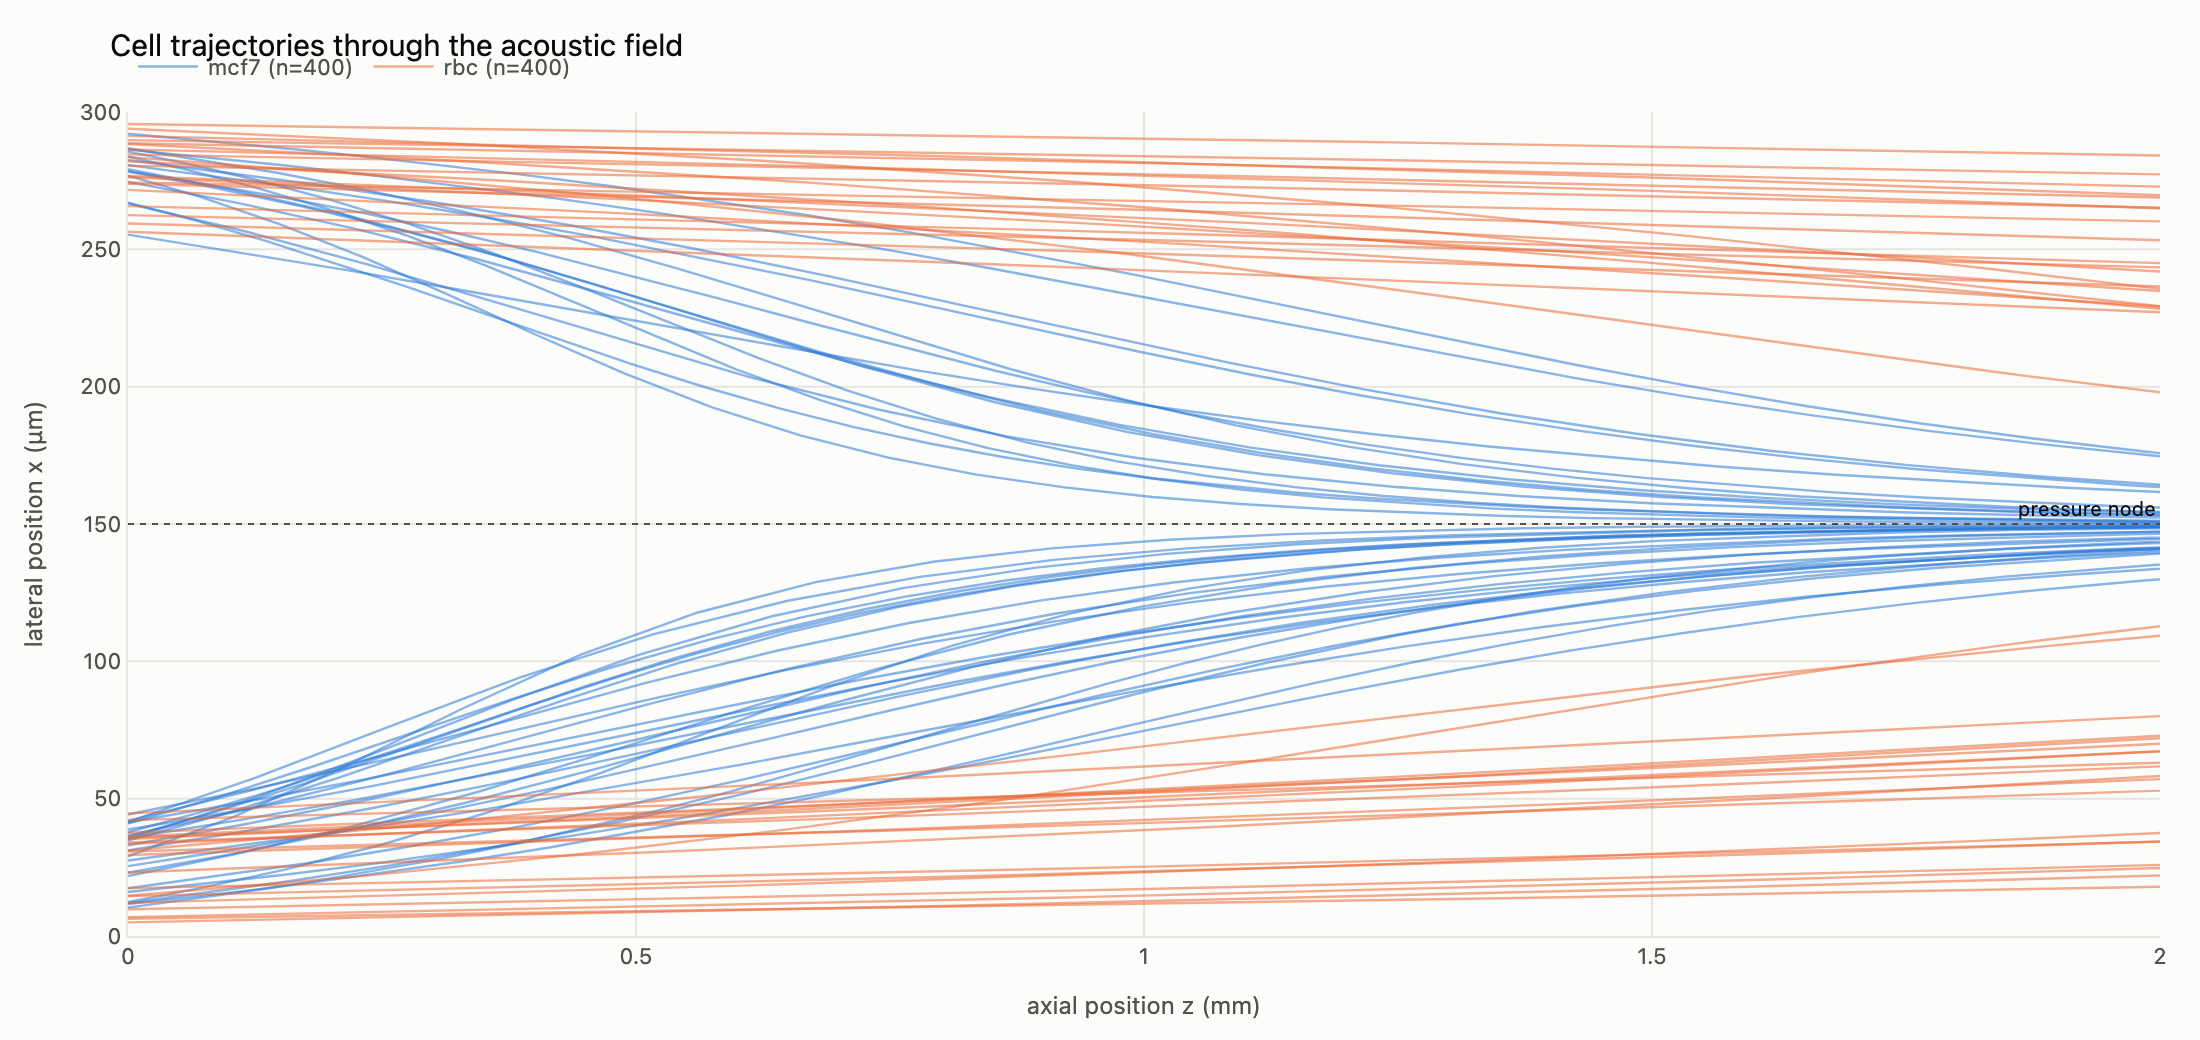
\includegraphics[width=0.94\textwidth]{../../assets/02_trajectories.png}
\caption{$r^2$ yasası, simüle edilmiş. 400 tümör hücresi (mavi) ve 400 alyuvar
(turuncu) iki duvardan girer ve kanal boyunca \SI{2}{\milli\meter} yol alır; bu
\SI{0,36}{\second} sürer. Tümör hücreleri ortaya ulaşır; alyuvarlar neredeyse
hiç kımıldamaz. Bu cihazda başka hiçbir şey olmuyor.}
\end{figure}

Kontrast faktörünün aslında bize \emph{karşı} çalıştığına dikkat edin ---
alyuvarın $\Phi$'si daha yüksektir (0,252'ye karşı 0,179), çünkü suya göre bir
tümör hücresinden daha yoğun ve daha serttir. Boyut yine de onu ona bir ezer.

\section{Ses nereden geliyor: çip üzerinde bir deprem}

\SI{300}{\micro\meter} genişliğinde bir kanalın içinde duran bir ses dalgasına
ihtiyacımız var. Hoparlöre yer yok. Bunun yerine kanal, \textbf{lityum niyobat}
adlı bir kristal levhanın üzerine oturur; bu kristal \emph{piezoelektriktir}:
gerilim uygularsanız fiziksel olarak biçim değiştirir, biçimini değiştirirseniz
gerilim üretir.

O kristalin yüzeyine iç içe geçmiş iki metal tarak yatırırız; bunlara
\textbf{arayüzlü dönüştürücü} ya da IDT denir. Taraklar arasına alternatif
gerilim uygulayın, kristal dalgalanır --- yalnızca üst yüzeyle sınırlı, küçük ve
son derece hızlı bir deprem. Buna \textbf{yüzey akustik dalgası} denir.

\begin{figure}[h]
\centering
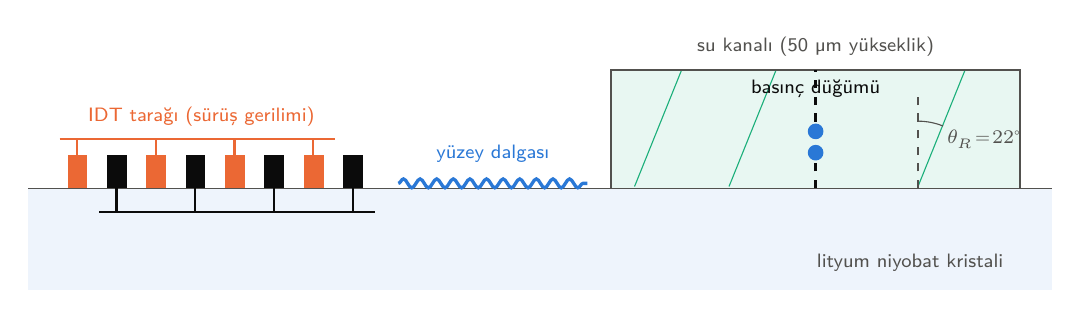
\begin{tikzpicture}[x=1cm,y=1cm]
  \fill[blue1!8] (0,-1.3) rectangle (13,0);
  \draw[muted] (0,0) -- (13,0);
  \node[font=\scriptsize\sffamily,color=muted] at (11.2,-0.95)
        {lityum niyobat kristali};
  \foreach \x in {0.5,1.5,2.5,3.5}{
    \fill[orange1] (\x,0) rectangle (\x+0.25,0.42);}
  \foreach \x in {1.0,2.0,3.0,4.0}{
    \fill[ink] (\x,0) rectangle (\x+0.25,0.42);}
  \draw[orange1,thick] (0.4,0.62) -- (3.9,0.62);
  \foreach \x in {0.5,1.5,2.5,3.5}{\draw[orange1,thick] (\x+0.12,0.42)--(\x+0.12,0.62);}
  \draw[ink,thick] (0.9,-0.3) -- (4.4,-0.3);
  \foreach \x in {1.0,2.0,3.0,4.0}{\draw[ink,thick] (\x+0.12,0)--(\x+0.12,-0.3);}
  \node[font=\scriptsize\sffamily,color=orange1,above] at (2.2,0.66)
       {IDT tarağı (sürüş gerilimi)};
  \draw[blue1,very thick,decorate,
        decoration={snake,amplitude=1.6pt,segment length=6pt}] (4.7,0.06) -- (7.1,0.06);
  \node[font=\scriptsize\sffamily,color=blue1,above] at (5.9,0.2) {yüzey dalgası};
  \fill[aqua1!10] (7.4,0) rectangle (12.6,1.5);
  \node[font=\scriptsize\sffamily,color=muted,above] at (10,1.55)
       {su kanalı (50 µm yükseklik)};
  \begin{scope}
    \clip (7.4,0) rectangle (12.6,1.5);
    \foreach \x in {7.7,8.9,11.3}{
      \draw[-{Stealth[length=4pt]},aqua1] (\x,0.02) -- ++(68:1.9);}
  \end{scope}
  \draw[muted,thick] (7.4,0) -- (7.4,1.5) -- (12.6,1.5) -- (12.6,0);
  \draw[muted,dashed] (11.3,0) -- (11.3,1.25);
  \draw[muted] (11.3,0.85) arc (90:68:0.85);
  \node[font=\scriptsize,color=muted,right] at (11.55,0.62) {$\theta_R\!=\!22^\circ$};
  \draw[ink,very thick,dashed] (10,0) -- (10,1.5);
  \node[font=\scriptsize\sffamily,color=ink,above] at (10,1.02)
       {\,basınç düğümü\,};
  \node[circle,fill=blue1,inner sep=2pt] at (10,0.45) {};
  \node[circle,fill=blue1,inner sep=2pt] at (10,0.72) {};
\end{tikzpicture}
\caption{Cihazın kesiti. Tarak biçimli bir elektrot kristal yüzeyi boyunca bir
dalgalanma sürer. Dalgalanma kristalde (\SI{3979}{\meter\per\second}) sesin
suda gittiğinden (\SI{1497}{\meter\per\second}) daha hızlı gittiği için, sıvıya
sabit bir açıyla, yaklaşık $22^\circ$ ile sızar --- bir bardak sudaki pipetin
kırık görünmesiyle aynı nedenle. Karşılıklı iki yönden gönderilen iki böyle
dalga duran örüntüyü oluşturur.}
\end{figure}

Sızma açısını, suya giren ışığı büken kuralın aynısı belirler:

\begin{equation}
\theta_R = \arcsin\!\left(\frac{c_{\text{su}}}{c_{\text{SAW}}}\right)
= \arcsin\!\left(\frac{1497}{3979}\right) = 22{,}1^\circ
\end{equation}

Bu açıyı simülasyona biz koymuyoruz. Bilgisayara kristal yüzeyinin ne yaptığını
söylüyor, sudaki ses denklemini çözmesini istiyoruz ve $22^\circ$ kendiliğinden
çıkıyor. Bu, fiziğin varsayılmak yerine çözüldüğünün küçük ama gerçek bir
göstergesidir.
